\section{Introduction}

Explaining the decisions of a trained neural network is among the deepest questions in machine learning.
Several methods have been proposed to make these decisions more interpretable, 
including visualization and computing several metrics. 
We present a technique to boost various of these approaches. 
The basic idea is to split a trained neural network in two (convex) monotone networks, allowing to benefit from the better interpretability of the latter type of networks. 
Explainability is crucial for debugging and improving models, detecting spurious correlations, and fostering trust in deployment. 
Methods of explainable artificial intelligence (XAI) have been used to localize relevant evidence, diagnose failure modes, and validate the reliability of explanations themselves \citep{ZeilerFergus2014,Montavon2017DeepTaylor,Ribeiro2016,Adebayo2018,Anders2020ClArC}. 

\begin{figure}[htbp]
    \centering
    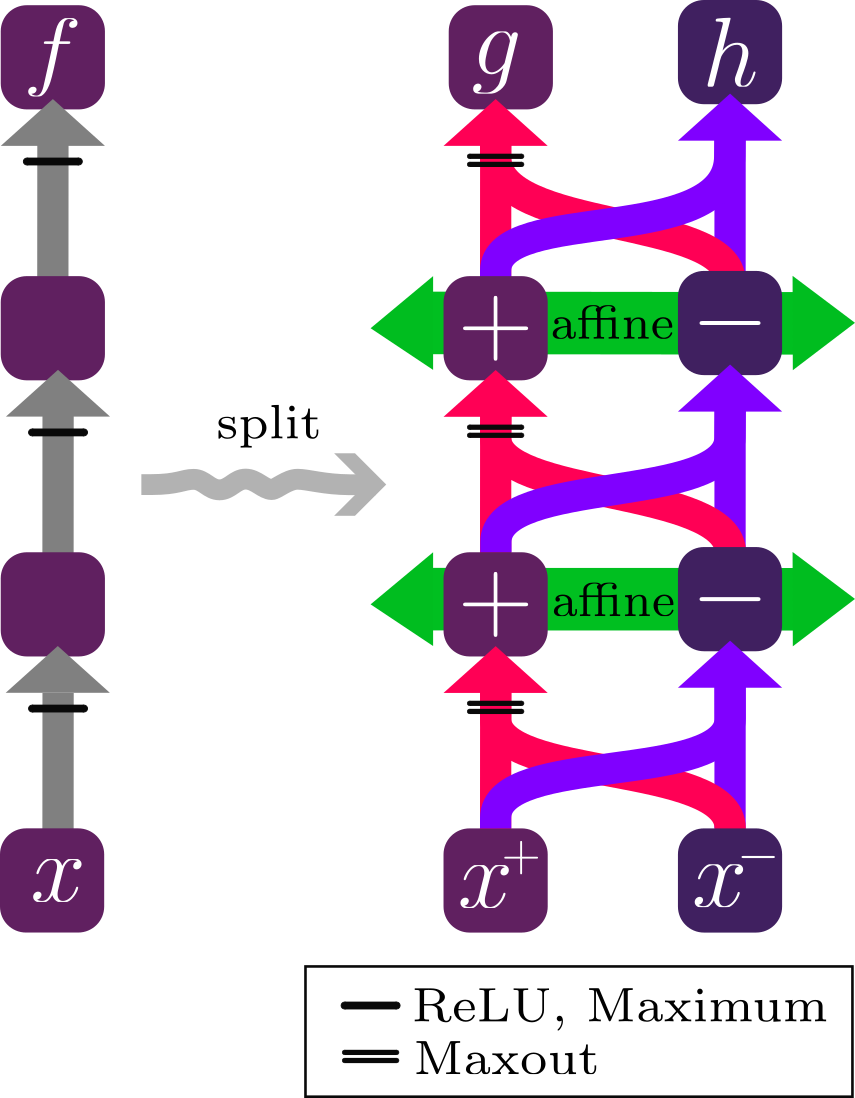
\includegraphics[width=0.28\textwidth]{figures/network_split.png}
    \caption{Illustration of the network splitting procedure. A ReLU network $f$ is decomposed into two monotone and convex streams $g$ and $h$, such that $f = g - h$.}
    \label{fig:network_split}
\end{figure}

\paragraph{Monotonicity as a tool for XAI}
Monotonicity has long been associated with interpretability, (adversarial) robustness, and fairness in machine learning \citep{Amos2017,Wang2020ShapeFairness,Liu2020CertifiedMonotone}. 
Networks that enforce non-negative weights
have been demonstrated to correctly express monotone dependences
and represent actual parts of the learned structure as no cancellation can arise~\citep{ayinde2018nonnegativity,lee1999nmf}.
However, while these models offer interpretability and fairness “by design”, they typically come at a cost in expressivity and cannot be easily applied to existing pretrained architectures.
In this work, we address this issue.
We use the idea of splitting any ReLU network into a pair of two \emph{split-streams}, structured sub-networks with non-negative weights, both representing monotone and convex functions $g$ and $h$ such that the originally represented function $f$ is their difference $f=g - h$ (see \cref{fig:network_split}).
The key idea arises from the identity
\begin{align}
    \relu(a-b) = \max\{a-b,0\} = \max\{a,b\} - b \enspace \label{eq:max_formulation}.
\end{align}
While this splitting was already present in earlier work~\citep{Siahkamari2020_DCRegression,Awasthi2023DCNN} as a special case of a Difference-of-Convex Decomposition (DC Decomposition), it has not been successfully applied in the context of explainability.
Our key contribution lies in the numerical stabilization of the forward and backward pass through this split representation by affine transformations of network activations and gradients.
This allows us to use it effectively as a tool for increasing explainability of an already trained model without retraining or altering predictions. 
Intuitively, the distinct positive and negative split-streams of the \emph{split-pair} preserve pre-activation information even when the original neuron output is zero. 

\paragraph{SplitCAM and SplitLRP}
Concretely, we develop a LayerCAM-inspired saliency method on this representation \citep{Jiang2021LayerCAM} and furthermore adapt Layer-wise Relevance Propagation to operate on the split-pair~\citep{Bach2015}.
Evaluated on VGG16~\citep{Simonyan2015} and ResNet18~\citep{Kaiming2016_resnet} with Quantus~\citep{Hedstrom2023}, the split methods show configuration-dependent gains in localization and Selectivity, with trade-offs in Pixel Flipping and robustness. These results measure distinct properties of the attribution maps; localization gains alone do not establish greater faithfulness to the model's decision process.
In some sense, the split-pair enforces a monotone, biologically plausible computational scheme:
non-negative activations and weights allow neurons only to increase evidence for a class rather than inhibit it, mirroring biological neural processing~\citep{lee1999nmf,Dayan2001_TheoreticalNeuroscience}.

\paragraph{Differences of networks}
One may ask whether the observed gradient patterns of split models also arise in directly trained differences of constrained networks.
We therefore complement the post hoc splitting study by training differences of convex or monotone networks directly.

We train DIC-models (difference-of-convex) and DM-models (difference-of-monotone). 
When the input to the $h$-stream is inverted, the displayed MNIST examples show class-dependent
stream sensitivities on present strokes and candidate missing-stroke locations, see
\cref{app:explaining_io_convex_nns}. These qualitative patterns motivate a factual/counterfactual
interpretation to be tested through interventions on the complete model; either stream alone
does not determine the effect of an input change on the model's output.

\paragraph{Related work on convexity / monotonicity} 
DC-decompositions of neural networks have already appeared in various work. 
Most notably, the decomposition of a feedforward as well as convolutional neural network was presented in~\citep{Awasthi2023DCNN} so that DC-programming could be applied to train a network. On the other hand, using quadratic programming, basically the same decomposition was used in~\citep{Siahkamari2020_DCRegression} to efficiently fit a difference of convex functions to data. 
Additionally, \citep{Sankaranarayanan2021CDINN} introduce the network architecture based on a difference of two convex functions (CDiNN) and show that it behaves well for optimal control problems.  
More generally, there is a lot of work on finding and leveraging DC-decompositions in optimization~\citep{Melzer1986_PLasDC,Kripfganz1987_PWAasDC,Zalgaller2000_DCRepresentation,Griewank2020_PolyhedralDCDecomposition,Schlueter2021_ConvexDecompPAF,Koutschan2024_MinimalArity,Kazda2024_LP_DCPLA,Brandenburg2025_DecompositionPolyhedra}.
As a building block, it is important to mention the fundamental idea to use (partially) monotone networks, going back to~\citep{Sill1997_MonotonicNetworks}
and appearing in various contexts~\citep{Sivaraman2020_COMET,sivaprasad2021curious,Nguyen2023_MonoNet,Liu2020CertifiedMonotone,Daniels2010_MonotoneNN}.
While these are usually based on non-negative weights, the class of input convex neural networks (ICNN) is similar but more general~\citep{Amos2017}.

\paragraph{Related work on XAI} 
A large body of XAI research investigates pixel- or feature-level attributions in deep networks, including gradient saliency~\citep{Simonyan2014}, deconvolutional and guided-backprop visualizations~\citep{ZeilerFergus2014,Springenberg2015}, Layer-wise Relevance Propagation (LRP) and deep Taylor decomposition~\citep{Bach2015,Montavon2017DeepTaylor}, class-activation mapping (Grad-CAM)~\citep{Selvaraju2017}, axiomatic attributions such as Integrated Gradients and DeepLIFT~\citep{Sundararajan2017,Shrikumar2017}, noise-averaged gradients (SmoothGrad)~\citep{Smilkov2017}, and perturbation- or surrogate-based explanations (LIME, Meaningful Perturbations, SHAP, EVA, SharletX)~\citep{Ribeiro2016,FongVedaldi2017,LundbergLee2017, Kolek2023_ShearletX, Fel2023_EVA}.
Such tools have exposed spurious “Clever Hans” behaviors and guided mitigation strategies \citep{Anders2020ClArC,Kauffmann2020CleverHans,Kauffmann2018OneClassDTD}.

\paragraph{Contributions}
Our main contributions are as follows:
\begin{itemize}
    \item \textbf{A numerically stable DC decomposition of ReLU networks, including CNNs.}
    We propose an algorithm that transforms any pretrained ReLU network into two monotone and convex subnetworks without altering its outputs. This includes novel stabilization techniques for both the forward and backward pass.
    
    \item \textbf{New attribution methods — SplitCAM, SplitLRP, and SplitGrad.}
    We adapt LayerCAM and LRP to operate on the split networks and introduce a new gradient-based method, leveraging the improved signal flow in the DC Decomposition.
    
    \item \textbf{Attribution benchmarks and stabilization ablations.}
    Across VGG16 and ResNet18 on ImageNet-S~\citep{Gao2022imagenets}, our methods show metric- and configuration-dependent gains on the Quantus benchmark suite. Guided Grad-CAM retains the highest reported Attribution Localization on ResNet18, and SplitCAM's Selectivity advantage over Guided Backprop is $0.014$. The ablations characterize how the choice of layer, split-stream rule, and stabilization parameter changes localization, perturbation scores, and robustness.
\end{itemize}
